\documentclass{article}
\usepackage{blindtext}
\usepackage{booktabs}
\usepackage{subcaption}
\usepackage{graphicx}
\usepackage{caption}
\usepackage{hyperref}
\usepackage{pdflscape}
\usepackage{tikz}
\usepackage{threeparttable}
\usepackage{algorithmic}
\usepackage[margin=0.25in]{geometry}
\usepackage{amsfonts}
\usepackage{amsmath,amssymb}
\usepackage{amsthm}
\usepackage{mathtools}

\title{EC709 PS1}
\author{Everett Stamm}
\begin{document}
\maketitle
\section*{Note}
I can't actually figure out how to export glmnet or locfit results to a latex table so I'm just describing them in this document. All results can be found in code.R or on \url{https://github.com/everettstamm1/EC709_PS1}
\section{Question 1}
\subsection{Part 1}
Omitted.
\subsection{Part 2}
From the slides, recall that
\[
\hat{g}_h(x) = e_1'(X'W X)^{-1}X'WY
\]
Where $e_1$ is $(r+1) \times 1$ vector with $1$ in the first entry and zeros elsewhere and $W = diag(K_h(x-X_1), \dots, K_h(x - X_n))$. Add and subtract a $g_0 = (g_0(X_1), \dots, g_0(X_n))'$ to this and square to get MSE:
\[
MSE = E[(\hat{g}_h(x) - g_0(x))^2 | X_i ] = e_1'(X'WX)^{-1}X'W \Sigma W X (X'WX)^{-1} e_1 + \Big(e'_1 (X'WX)^{-1}X'Wg_0 - g_0(x)\Big)^2
\]
Where the first term is the variance and the second is the bias squared. Also $\Sigma$ is an $N \times N$ diagonal matrix of the sample variances: $\Sigma = diag(\sigma^2(X_1), \dots, \sigma^2(X_n))$

 Not get taylor approximation of $g(X_i)$
\[
g(X_i) \approx g_0(x) + g_0'(x)(X_i - x) +(1/2) g_0''(x)(X_i-x)^2
\]
Rename $r_i =(1/2) g_0''(x)(X_i - x)^2 = g_0(X_i) - g_0(x) - g_0'(x)(X_i - x)$. Thus we can rewrite:
\begin{align*}
	g_0(X_i) = g_0(x) - g_0'(x)(X_i - x) + r_i
\end{align*}
Since $X e_1 = (1, \dots, 1)'$ and $X e_2 = (X_1 - x, \dots, X_n - x)'$, we can write the above in vector form:
\[
g_0 =X e_1 g_0(x) - X e_2 g_0'(x) + r
\]
And substitute into the equation for bias 
\begin{align*}
Bias = e_1'(X'WX)^{-1}X'Wg_0 - g_0(x) =  \\
e_1'(X'WX)^{-1}X'W(X e_1 g_0(x) - X e_2 g_0'(x) + r) - g_0(x) = e_1'(X'WX)^{-1}X'Wr
\end{align*}

Now we need a corrolary: from the "weighted average" section of the notes we can see that
\[
S_j = W ((x - X^j)^j) / h^j \sum_i K_h(x - X_i)(\frac{x - X_i}{h})^j
\]
Multiply, divide, do a change of variables $u = (x - x_i)/h$ and take the expectation to get that 
\[
E[S_j/(n h^j)] = \mu_j f_0(x) + o(1)
\]
For $\mu_j = \int u^j K(u) du$. Note that the asymptotic variance of this can be shown to have
\[
Var(S_j/(n h^j)) = E[(S_j/(n h^j))^2] - (E[S_j/(n h^j)])^2 \leq  E[(S_j/(n h^j))^2] 
\leq \frac{1}{nh} \int u^{2j} K(u)^2 j_0(x - hu) du 
\]
The integral approaches some constant as $h \rightarrow 0$ and then $\frac{1}{nh} \rightarrow 0 $ as $nh \rightarrow \infty$, so the variance approaches zero. So we have that
\[
S_j/(nh^j) \rightarrow \mu_j f_0(x)+o(1)
\]
Now let $H = diag(1,h)$, so we have
\[
n^{-1} h^{-2} H^{-1} X' W r = n^{-1} h^{-2} H^{-1} X' S_2 (1/2) g_0''(x) \rightarrow (1/2) f_0(x) \begin{pmatrix} \mu_2 \\ 0 \end{pmatrix} g_0''(x) 
\]

We also have that as $h \rightarrow 0$ and $nh \rightarrow \infty$ 
\[
n^{-1}H^{-1}X' W X H^{-1} = n^{-1} \begin{bmatrix}
S_0 & h^{-1} S_1 \\
h^{-1} S_1 & h^{-2} S_2
\end{bmatrix} \rightarrow f_0(x) \begin{bmatrix}
 \mu_0 & \mu_1 \\
\mu_1 & \mu_2
\end{bmatrix}  = f_0(x) \begin{bmatrix}
 1 & 0 \\
0 & \mu_2
\end{bmatrix} 
\]

Now rearrange the bias equation
\begin{align*}
e_1'(X'WX)^{-1}X'Wr = e'_1 h^2 H^{-1} (n^{-1}H^{-1} X'W X H^{-1})^{-1} n^{-1} h^{-2} H^{-1} X' W r \rightarrow e'_1 h^2 H^{-1}\Big(f_0(x) \begin{bmatrix} 1 & 0 \\ 0 & \mu_2 \end{bmatrix} \Big)^{-1} (1/2) f_0(x) \begin{pmatrix} \mu_2 \\ 0 \end{pmatrix} g_0''(x) = \\
g''_0(x) (h^2/2)e_1' H^{-1} \frac{1}{\mu_2}\begin{bmatrix} \mu_2 & 0 \\ 0 & 1 \end{bmatrix} \begin{pmatrix} \mu_2 \\ 0 \end{pmatrix} = g''_0(x)(h^2/2) \mu_2 + o(1)
\end{align*}
Forgot the $o(1)$ along the way but here it is again.

Using what we learned for the bias, let's identify a new quantity:
\[
Q_j = \frac{h}{n} \sum_i K(x - X_i)^2 (\frac{x - X_i}{h})^j \sigma^2(x_i)
\]
Thus with change of variables $u = (x - X_i)/h$
\[
E[Q_j] = E[h K_h(x - X_i)^2  (\frac{x - X_i}{h})^j \sigma^2(x_i) ] = f_0(x) \sigma^2(x) \int u^j K(u)^2 du = f_0(x) \sigma^2(x) v_j
\]
Turns out that
\[
n^{-1} h H^{-1} X' W \Sigma W X H^{-1} = \begin{bmatrix} Q_0 & 0 \\ 0 & Q_2 \end{bmatrix}
\]
So then the variance equation becomes
\begin{align*}
e_1'(X'WX)^{-1}X'W \Sigma W X (X'WX)^{-1} e_1 = n^{-1}h^{-1}e'_1 H^{-1} \Big(\frac{H^{-1} X' W X H^{-1}}{n}\Big) \Big(\frac{h H^{-1} X'W \Sigma W X H^{-1}}{n} \Big) \Big(\frac{H^{-1} X' W X H^{-1}}{n}\Big)H^{-1} e_1 \rightarrow \\
n^{-1} h^{-1}e_1'(f_0(x) \begin{bmatrix} 1 & 0 \\ 0 & \mu_2 \end{bmatrix})^{-1} \begin{bmatrix} Q_0 & 0 \\ 0 & Q_2 \end{bmatrix}(f_0(x) \begin{bmatrix} 1 & 0 \\ 0 & \mu_2 \end{bmatrix})^{-1}e_1 = n^{-1}h^{-1} \frac{v_0 \sigma^2(x)}{f_0(x)} + o(1)
\end{align*}
\subsection{Part 3}
Below is the table of simulated values. 

% Table created by stargazer v.5.2.3 by Marek Hlavac, Social Policy Institute. E-mail: marek.hlavac at gmail.com
% Date and time: Tue, Sep 17, 2024 - 8:36:30 PM
\begin{table}[!htbp] \centering 
  \caption{} 
  \label{} 
\begin{tabular}{@{\extracolsep{5pt}} cccccc} 
\\[-1.8ex]\hline 
\hline \\[-1.8ex] 
 & h & kern\_bias & kern\_var & local\_bias & local\_var \\ 
\hline \\[-1.8ex] 
1 & $0.050$ & $0.013$ & $0.142$ & $0.018$ & $0.150$ \\ 
2 & $0.100$ & $0.015$ & $0.120$ & $0.011$ & $0.143$ \\ 
3 & $0.150$ & $0.014$ & $0.100$ & $0.012$ & $0.137$ \\ 
4 & $0.200$ & $0.010$ & $0.079$ & $0.019$ & $0.136$ \\ 
\hline \\[-1.8ex] 
\end{tabular} 
\end{table} 

\subsection{Part 4}
Asymptotic theory would predict the following for local linear regression:
\[
E[Bias] = E[g_0''(x)(h^2/2)\mu_2] = E[\exp(X)(h^2/2) (1/5)] = (h^2/2) (1/5)(\exp(1) - \exp(0))
\]
Thus for $h = (0.05,0.1,0.15,0.2)$ we'd expect $Bias = (0.0004,0.0017,0.0039,0.0067)$. Kinda makes sense that since we're holding $n$ constant while $h \rightarrow 0$, the values get further from their true value. Similarly:
\[
E[Variance] =E[ \frac{1}{1000h}\frac{(3/5) \sigma^2(x)}{ f_0(x)}] = \frac{1}{1000h}\frac{(3/5) 0.5^2/12}{1}
\]
 Thus for $h = (0.05,0.1,0.15,0.2)$ we'd expect $Variance = (0.00025, 0.000125,0.000083,0.0000625)$. Clearly we're very far off!
\section{Question 2}

\subsection{Part 1}
In code.R, I optimized the local linear regression over bandwidth values of $(0.1,0.2,0.3,0.4,0.5,0.6,0.7,0.8)$ and the power and bspline regressions over 1-7 knots. The optimal values were 0.1 for local linear, 7 for power, and 1 for bspline.
\begin{figure}
	\centering
	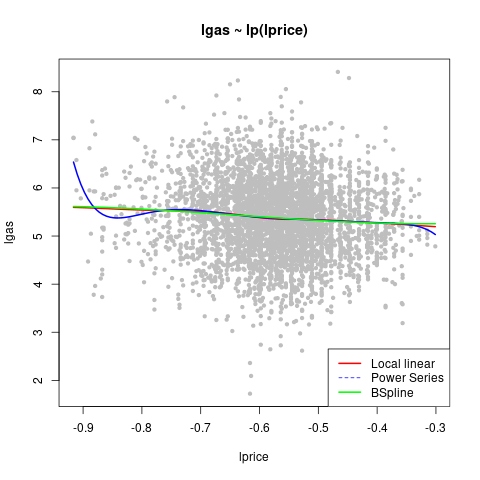
\includegraphics{Q2_1.png}
\end{figure}
\subsection{Part 2}
With the price set to 0.57. I get betas of 5.34, 5.36, and 5.37 with standard errors of 0.02 0.016, and 0.013 for local linear, power, and bspline regressions, respectively.
\subsection{Part 3}
Again in code.R, I optimized the local linear regression over bandwidth values of $(0.1,0.2,0.3,0.4,0.5,0.6,0.7,0.8)$ and the power and bspline regressions over 1-7 knots. The optimal values were 0.1 for local linear, 7 for power, and 1 for bspline.
\subsection{Part 4}
In the standard lasso, the coefficient on log price is $-0.554$, while in the two-way one it's fixed at zero. That said, there are coefficients of -0.253, -0.057, and 0.125 on the interaction of log price and driver, hhsize, and urban, respectively.
\section{Question 3}
Below is the prediction error for the 5 estimators. Clearly, there are benefits to cross validation, though surprisingly post lasso CV is higher than just the lasso CV. 

% Table created by stargazer v.5.2.3 by Marek Hlavac, Social Policy Institute. E-mail: marek.hlavac at gmail.com
% Date and time: Thu, Sep 19, 2024 - 10:40:01 AM
\begin{table}[!htbp] \centering 
  \caption{} 
  \label{} 
\begin{tabular}{@{\extracolsep{5pt}}lccccc} 
\\[-1.8ex]\hline 
\hline \\[-1.8ex] 
Statistic & \multicolumn{1}{c}{N} & \multicolumn{1}{c}{Mean} & \multicolumn{1}{c}{St. Dev.} & \multicolumn{1}{c}{Min} & \multicolumn{1}{c}{Max} \\ 
\hline \\[-1.8ex] 
lasso\_pe & 500 & 5.917 & 0.829 & 3.657 & 9.089 \\ 
post\_lasso\_pe & 500 & 2.871 & 0.394 & 1.696 & 4.140 \\ 
lassoCV\_pe & 500 & 0.258 & 0.130 & 0.039 & 0.934 \\ 
post\_lassoCV\_pe & 500 & 0.562 & 0.246 & 0.027 & 1.300 \\ 
oracle\_pe & 500 & 0.061 & 0.036 & 0.006 & 0.278 \\ 
\hline \\[-1.8ex] 
\end{tabular} 
\end{table} 

\end{document}